\chapter{\hminus\ AND MOLECULES}
% !TEX root = hazy3.tex

\section{Overview}

An ion-molecule network, initially based on \citet{Black1978} but heavily
revised to include a large network, is included in \Cloudy.  Aspects are
discussed in \citet{Ferland1989}, \citet{Ferland1994},
\citet{FerlandFabian2002}, \citet{Henney2005}, and \citet{Abel2005}.
\citet{Roellig2007} present
the results of a workshop that compared various codes' predictions of
conditions in atomic and molecular clouds.

\section{The Saha equation for arbitrary systems}

The Boltzmann equation relates the densities of related species by the
expression
\begin{equation}
\label{eqn:BoltzmannPopulations}
\frac{{{n_{final}}}}{{{n_{initial}}}} = \frac{{{\rho _{final}}}}{{{\rho
_{initial}}}}\exp \left( { - \Delta E/kT} \right)
\end{equation}
where $n_{initial}$  and $n_{final}$  indicate the densities of the initial and final
states, and the $\rho$'s are the densities of available states at a given energy.
Consider the process $i \Rightarrow j+k$.  The energy change during this process is
\begin{equation}
\Delta E = {\chi _I} + \frac{1}{2}m{v^2}
\end{equation}
where the first term is the ionization or dissociation potential of the
initial system, and the second term represents the kinetic energy of the
system in the final state.  The sign of $\Delta E$ is related to the energies of
the initial and final systems~by
\begin{equation}
{E_{final}} = {E_{initial}} + \Delta E.
\end{equation}
The $\rho$'s entering equation 1 are the total densities of states accessible
at an energy $E$.  Since the initial state is a bound particle we can take
it as at rest in the lab frame, and consider the final state consisting
of two constituent particles moving with kinetic energy $\Delta$E.  The density
of states of the final particles can be written as the product of densities
of states due to electron spin and to motion of the particle.  Nuclear spins
are assumed to be uncorrelated, so nuclear statistical weights cancel out
and are not carried through.

Considering only spin and motion (momentum) the total density of states
is the spin statistical weight of the particle $g_{spin}$ multiplied by the
density of states due to momentum $g_p$ (\citealp{Mihalas1978}, p 112; \citealp{Elitzur1992},
p 14):
\begin{equation}
{\rho _{total}} = {g_{spin}}{g_p}
\end{equation}
where $g_p$ is
\begin{equation}
{g_p} = \frac{{dx\,dy\,dz\,d{p_x}\,d{p_y}\,d{p_z}}}{{{h^3}}}.
\end{equation}
The volume element can be removed from the problem by defining it as the
volume containing one particle,
\begin{equation}
dx\,dy\,dz = {\left( {{n_k}/{g_k}} \right)^{ - 1}}
\end{equation}
while the momentum volume element is given in terms of the particle's speed
$u$ by
\begin{equation}
\label{eqn:MomentumVolume}
d{p_x}\,d{p_y}\,d{p_z} = 4\pi {p^2}\,dp = 4\pi \,{m^3}{u^2}\,du.
\end{equation}
Combining these with equation \ref{eqn:BoltzmannPopulations} we find
\begin{equation}
\frac{{{n_{final}}{n_k}}}{{{n_{initial}}}} = \frac{{{n_j}{n_k}}}{{{n_i}}}
= \left( {\frac{{{g_{spin,j}}{g_{spin,k}}}}{{{g_{spin,i}}}}} \right)\left(
{\frac{{{g_{p,j}}{g_{p,k}}}}{{{g_{p,i}}}}} \right)\exp \left( { - \Delta
E/kT} \right).
\end{equation}
Shortening $g_{spin,x}$ to simply $g_x$, and using equation \ref{eqn:MomentumVolume}, we find
\begin{equation}
\frac{{{n_j}{n_k}}}{{{n_i}}} = \left( {\frac{{{g_j}{g_k}}}{{{g_i}}}}
\right)\left( {\frac{{4\pi }}{{{h^3}}}\frac{{m_j^3u_j^2{\kern 1pt} \exp
\left( { - \frac{1}{2}{m_j}u_j^2/kT} \right)d{u_j}\,m_k^3u_k^2
\exp \left( { - \frac{1}{2}{m_k}u_k^2/kT} \right)d{u_k}}}{{\,m_i^3u_i^2 \exp \left( { - \frac{1}{2}{m_i}u_i^2/kT} \right)d{u_i}}}} \right)\exp \left( { - \Delta E/kT} \right)
\end{equation}
Integrating each energy term over velocity, making the substitution
\begin{equation}
x \equiv {\left( {\frac{m}{{2kT}}} \right)^{1/2}}u,
\end{equation}
we find
\begin{equation}
\int_0^\infty  {u_j^2{\kern 1pt} \exp \left( { - \frac{1}{2}{m_j}u_j^2/kT}
\right)d{u_j}{\kern 1pt} }  = {\left( {\frac{{2kT}}{{{m_j}}}}
\right)^{3/2}}\int_0^\infty  {\exp \left( { - {x^2}} \right){x^2}\,dx}
= {\left( {\frac{{2kT}}{{{m_j}}}} \right)^{3/2}}\frac{{{\pi ^{1/2}}}}{4}
\end{equation}
where the root $\pi$ over 4 is the value of the integral.  The final form of
the Saha equation, for an arbitrary system, is:
\begin{equation}
\begin{array}{ccc}
 \frac{{{n_j}{n_k}}}{{{n_i}}}& =& \left( {\frac{{{g_j}{g_k}}}{{{g_i}}}}
\right){\left( {\frac{{2\pi \,kT}}{{{h^2}}}\frac{{{m_j}{m_k}}}{{{m_i}}}}
\right)^{3/2}}\exp \left( { - \Delta E/kT} \right) \\
&=& 8.7819 \times {10^{55}}\left( {\frac{{{g_j}{g_k}}}{{{g_i}}}}
\right){\left( {\frac{{T{m_j}{m_k}}}{{{m_i}}}} \right)^{3/2}}\exp \left(
{ - \Delta E/kT} \right) \\
 \end{array}.
\end{equation}
For the case of ionization producing an electron, the mass of the electron
is neglected relative to the mass of the atom.  If the atom and ion are
$i$ and $j$, then we have a mass ratio factor that is basically
\begin{equation}
\frac{{{m_j}{m_k}}}{{{m_i}}} = \frac{{{m_{ion}}{m_e}}}{{{m_{atom}}}}
\approx {m_e}.
\end{equation}
The most common final expression (\citealp{Mihalas1978}) includes the assumption
that $m_i$ and $m_k$ are nearly identical, and cancel out.   In this case we obtain
the form of the Saha equation most often encountered for hot gas, with the
2 being the spin statistical weight of the electron:
\begin{equation}
\frac{{{n_{ion}}{n_e}}}{{{n_{atom}}}} = \left(
{\frac{{{g_{ion}}2}}{{{g_{atom}}}}} \right){\left( {\frac{{2\pi
\,{m_e}kT}}{{{h^2}}}} \right)^{3/2}}\exp \left( { - \Delta E/kT} \right).
\end{equation}
In the case of molecular hydrogen
\begin{equation}
\frac{{{n_{\mathrm{H}}}{n_{\mathrm{H}}}}}{{{n_{{{\mathrm{H}}_{\mathrm{2}}}}}}} = 4{\left(
{\frac{{\pi \,kT{m_p}}}{{{h^2}}}} \right)^{3/2}}\exp \left( { - \Delta E/kT}
\right).
\end{equation}

\section{LTE Populations of hydrogen molecules}

In much of the following discussion comparison and relationships will
be made between the predicted hydrogen species populations and their LTE
values.

The statistical weight of H$_2^+$ is 4 while that of H$_2$ is 1 and the
dissociation energies are 2.647 eV and 4.477 eV respectively.

The LTE relative population density of \hminus\ is
\begin{equation}
{P^*}\left( {{{\mathrm{H}}^ - }} \right) = \frac{{{n^*}\left( {{{\mathrm{H}}^
- }} \right)}}{{{n_e}n\left( {{{\mathrm{H}}^{\mathrm{0}}}} \right)}} =
\frac{{{g_{{{\mathrm{H}}^ - }}}}}{{{g_{{{\mathrm{H}}^{\mathrm{0}}}}}{g_e}}}{\left(
{\frac{{{h^2}}}{{2\pi \,{m_e}kT}}} \right)^{3/2}}\exp \left[ {I({{\mathrm{H}}^
- })/kT} \right]\quad  [\mathrm{cm}^3]
\end{equation}
where $g_i$ is the statistical weight of the constituents,
(${g_{{{\mathrm{H}}^{\mathrm{ - }}}}} = 1$; ${g_{{{\mathrm{H}}^{\mathrm{0}}}}} = 2$; and
${g_e} = 2$),  the binding energy of the negative hydrogen ion is $I$(\hminus) = 0.055502
Ryd, and other constants have their usual meaning.

The LTE relative population density of H$_2$ is
\begin{equation}
{P^*}\left( {{{\mathrm{H}}_2}} \right) = \frac{{{n^*}\left( {{{\mathrm{H}}_2}}
\right)}}{{n\left( {{{\mathrm{H}}^{\mathrm{0}}}} \right)n\left( {{{\mathrm{H}}^{\mathrm{0}}}}
\right)}} =
\frac{{{g_{{{\mathrm{H}}_2}}}}}{{{g_{{{\mathrm{H}}^{\mathrm{0}}}}}{g_{{{\mathrm{H}}^{\mathrm{0}}}}}}}{\left(
{\frac{{{h^2}}}{{\pi \,{m_p}kT}}} \right)^{3/2}}\exp \left[
{I({{\mathrm{H}}_2})/kT} \right] [\mathrm{cm}^3]
\end{equation}

\section{The \hminus\ balance; radiative processes}

Although only a trace amount of hydrogen is in the form of \hminus, the opacity
provided by this ion is often dominant in the optical and near infrared,
and it couples energy in the near infrared continuum to moderately ionized
gas.  The methods and approximations employed to include heating and cooling
by \hminus\ are described here. Other discussions can be found in
\citet{Lambert1968}, \citet{Vernazza1981}, and \citet{Lites1984}.
This section is based on \citet{Ferland1989}.

The equilibrium density of \hminus\  is determined by assuming statistical
equilibrium, and balancing production and destruction mechanisms.  Great
care is taken in including both forward and back reactions, to ensure that
the present treatment of \hminus\ is capable of going to LTE in the limit of high
radiation or particle densities.

\subsection{Radiative attachment}

This is the most important creation mechanism for \hminus\ at low densities,
when three-body processes are negligible;
\begin{equation}
{H^o} + {e^ - } \Rightarrow {H^ - } + \gamma \quad .
\end{equation}

For temperatures greater than $10^4 \K$ the rate coefficient is evaluated
by numerically integrating the photodetachment cross section over frequency;
\begin{equation}
{\alpha _{rad}}\left( T \right) = {P^*}\left( {{{\mathrm{H}}^ - }}
\right)\int_{{\nu _o}}^\infty  {{\alpha _\nu }\frac{{8\pi \,{\nu
^2}}}{{{c^2}}}\exp \left( { - h\nu /kT} \right)\;d\nu }\quad  [\mathrm{cm}^3
\mathrm{s}^{-1}]
\end{equation}
where cross sections computed by \citet{Wishart1979} and spline interpolation
are used.  These cross sections are in excellent agreement with the velocity
operator bound-free cross sections tabulated by \citet{Doughty1966}.
The energy interval between the photodetachment threshold at 0.055502 Ryd
and $\sim$1.8 Ryd is divided into a large number of cells with logarithmically
increasing width, and the integration is carried out as a straight forward
sum.

This method is not numerically expedient for very low temperatures, where
the energy bandwidth of the integral is small, and a much finer frequency
grid would be required.  Rather, the integration was carried out using spline
interpolation and 32 point gaussian quadrature, integrating over factors
of two in $h\nu/kT$.  The results were then fitted with a set of power-laws.
The rate coefficients can be approximated by:
\begin{equation}
\alpha(T)_e)=\left\{\begin{array}{lc}
8.934 \times 10^{18}T^{0.505}& 1K\le T < 31.62 K\\
5.159 \times 10^{18}T^{0.664}& 31.62K\le T < 90 K\\
2.042 \times 10^{18}T^{0.870}& 90K\le T < 1200 K\\
8.861 \times 10^{18}T^{0.663}& 1200K\le T < 3800 K\\
8.204 \times 10^{17}T^{0.303}& 3800K\le T < 10^4 K\\
\end{array}\right.\quad [\mathrm{cm}^3\; \mathrm{s}^{-1}]
\end{equation}
These approximations fit the exact numerical results with a mean deviation
of 0.7 percent, and the largest error of 2.05 percent, over the indicated
temperature range.

Tests show that the numerical radiative attachment rates computed here
are in very good agreement with the approximation given by \citet{Hutchings1976},
who used the cross sections computed by \citet{Doughty1966}, for
temperatures $500 \K \le T  \le 2500 \K$.  (Notice that there is a typographical error
in the approximation for the radiative attachment rate given by
\citet{Palla1983}.)  It is also within 10\% of the value given
by \citet{Dalgarno1963}, which was based on earlier calculations
of the photodetachment cross section.

Continuum occupation numbers can be large in the infrared.  The induced
radiative attachment rate coefficient is
\begin{equation}
{\alpha _{ind}}(T) = {P^*}({{\mathrm{H}}^ - })\int_{{\nu _o}}^\infty  {{\alpha
_\nu }\frac{{4\pi \,{J_\nu }(\tau )}}{{h\nu }}} \exp \left( { - h\nu /kT}
\right)\;d\nu \quad [\mathrm{cm}3 \mathrm{s}^{-1}]
\end{equation}
where the mean intensity of the depth-dependent continuum is $J_{\nu}(\tau)$.  This
expression is used for all temperatures.

\subsection{Photodetachment}

Photodetachment,
\begin{equation}
{{\mathrm{H}}^ - } + \gamma  \Rightarrow {{\mathrm{H}}^{\mathrm{0}}} + {e^ - },
\end{equation}
is the dominant \hminus\ destruction mechanism for many conditions.  The rate
is evaluated in the standard manner;
\begin{equation}
\Gamma \left( {{{\mathrm{H}}^ - }} \right) = \int_{{\nu _o}}^\infty  {{\alpha
_\nu }\left( {bf} \right)\frac{{4\pi \,{J_\nu }(\tau )}}{{h\nu }}} \;d\nu
\quad [\mathrm{s}^{-1}]
\end{equation}
The integral is evaluated as a sum over the numerically binned continuum.
The incident continuum is then attenuated by optical depth increments
\begin{equation}
d\tau ({{\mathrm{H}}^ - }) = {\alpha _\nu }(bf)\;n({{\mathrm{H}}^ - })\left\{
{1 - \exp \left( { - h\nu /kT} \right)/{b_{{{\mathrm{H}}^ - }}}}
\right\}\;f(r)\;dr
\end{equation}
where ${b_{\mathrm{H}^ - }}$
 is the departure coefficient for \hminus, ${b_{\mathrm{H}}^{ - }}$
$\equiv  n(\mathrm{H}^-)/n^*(\mathrm{H}^-), f(r)$ is the filling factor, and
$n^*$(\hminus) is the LTE \hminus\ density.

\subsection{Photodetachment by hard photons}

The \hminus\ photoabsorption cross section increases above  $\sim$3/4 Ryd, energies
where excitation of $n\ge  2$ levels is possible.  Cross sections that include
this process are taken from \citet{Broad1976}.  These calculations
do not extend to high energies, so I scaled high-energy hydrogen cross
sections by the ratio of \hminus\ to H$^o$ cross sections at 18\AA  in order to take
absorption of x- and $\gamma$- rays into account.

The cross section for ($\gamma$,2e$^-$) absorption is much smaller than
($\gamma$, e$^-$) \citep{Broad1976}, and this latter process is neglected.

\subsection{The approach to LTE; high radiation densities}

As a test of the assumptions and methods, the approach to LTE under
conditions determined by radiative attachment (spontaneous and induced)
and photodetachment are first considered.  Tests in which gas with
temperature $T$ is exposed to black body radiation fields with color
temperature $T_{color}$ are computed.  The color and gas temperatures are set
equal, $T = T_{color}$, and the intensity of the radiation field is varied up
to the black body limit.  The intensity of the radiation field is
parameterized by the equivalent energy density temperature $T_u =
(u/a)^{1/4}$,
where $u$ is the energy density (erg cm$^{-3}$; see above) and $a$ is the Stefan's
radiation density constant.  The equilibrium population of H- was computed,
including all process mentioned below, but with the hydrogen density small
enough (typically  10$^5$~cm$^{-3}$) for radiative processes to be most important.
The \hminus\ population is expressed as a departure coefficient, and the results
are shown in Figure \ref{fig:Hmi_vs_U}, for tests in which $T_{color} = 0.5, 1$, and
$2\times 10^4$~K.

\begin{figure}
\centering
\label{fig:Hmi_vs_U}
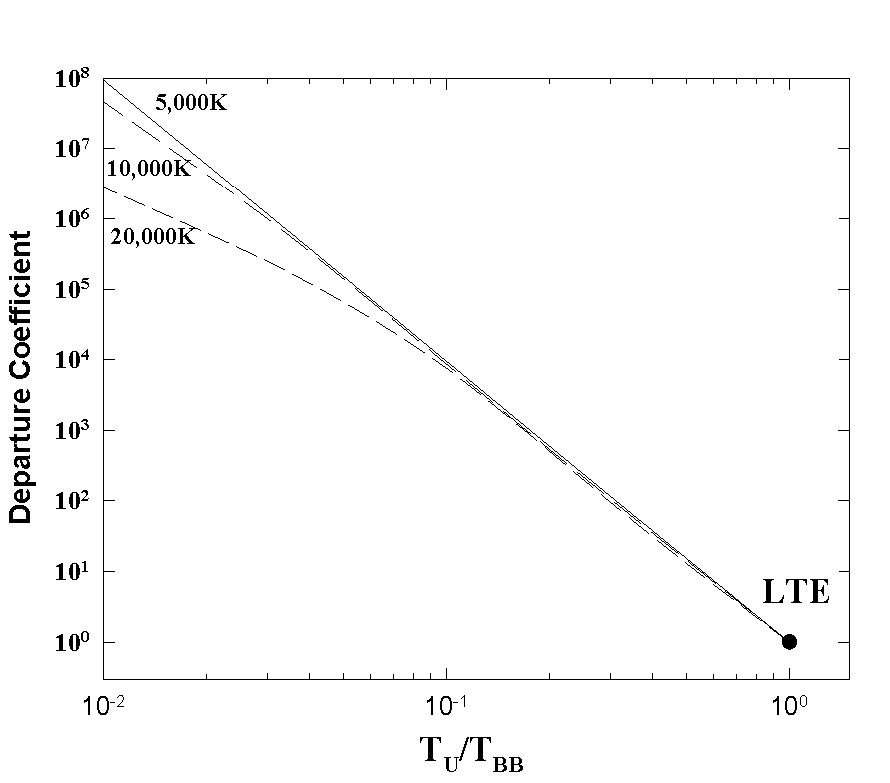
\includegraphics[scale=0.7]{Hmi_vs_U}
\caption[\hminus\ departure coefficients vs radiation energy density]{Departure coefficients for \hminus.  The figure shows tests in which
the hydrogen density was held fixed at a low and the gas irradiated by black
bodies with color temperatures of 5, 10, and $20 \times 10^3$ K.  Gas temperature
and color temperatures were equal. The energy density temperature $T_u$. was
varied up to its LTE limit.  The \hminus\ departure coefficient is within 0.2\%
of unity when $T_u = T_{color}$.}
\end{figure}

When $T_u = T_{color}$, and the radiation field is in strict thermodynamic
equilibrium, radiative processes must hold \hminus\ in LTE and departure
coefficients of unity are expected.  The computed departure coefficients
for the three temperatures are 0.9998, 0.9996, and 1.0030, respectively.
As the Figure shows, when $T_u$ is lowered below $T_{color}$, the intensity of the
radiation field falls below its thermodynamic equilibrium value, and the
population of \hminus\ increases.  This is because the photodetachment rate (which
is proportional to the intensity of the radiation field) is no longer in
balance with the radiative attachment rate (which is proportional only to
the electron density).

\section{The \hminus\ balance; collisional processes}

\subsection{Associative detachment}

The most important H$_2$ formation mechanism in grain-free environments,
and a significant \hminus\ destruction mechanism, is associative detachment,
\begin{equation}
{{\mathrm{H}}^ - } + {{\mathrm{H}}^0} \Leftrightarrow {{\mathrm{H}}_2} + {e^ - }
\end{equation}
where rate coefficients were originally from Bieniek and Dalgarno (1979)
and have been updated to \citet{Launay1991}.  The rate is shown in Figure
\ref{fig:hminus_to_h2}.  The reverse reaction rate $C_R$, for electron collisional dissociation
of H$_2$, is related to the forward rate coefficient $C_F$ by detailed balance;
\begin{equation}
{C_R} = {C_F}\frac{{{P^*}({{\mathrm{H}}^ - })}}{{{P^*}({{\mathrm{H}}_2})}}
\quad  [\mathrm{s}^{-1}].
\end{equation}

\begin{figure}
\centering
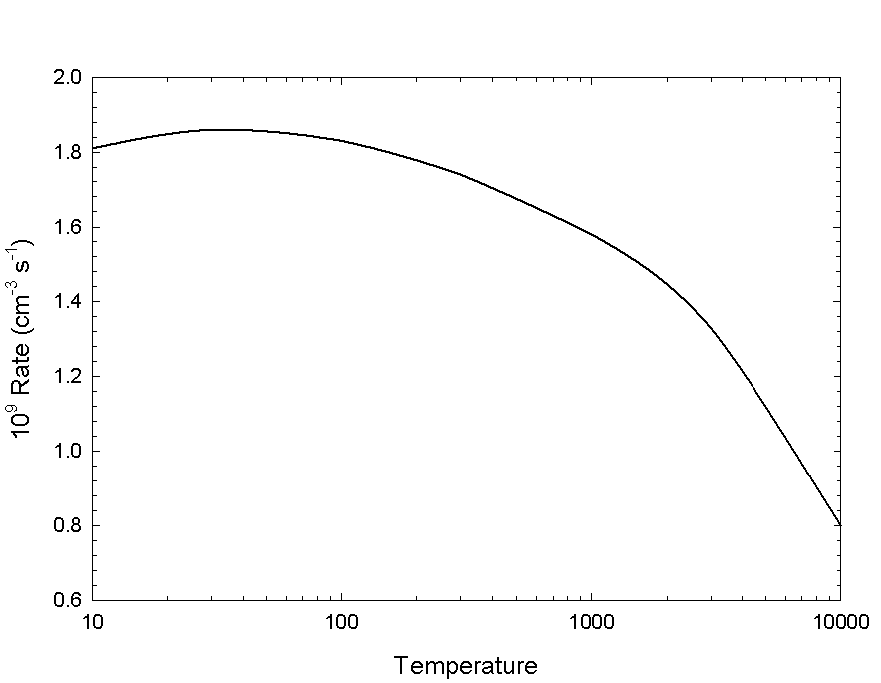
\includegraphics[scale=0.8]{hminus_to_h2}
\caption{Rate coefficient for H$^- \to \mathrm{H}_2$.
The rates are taken from Launay et al. (1991)}
\label{fig:hminus_to_h2}
\end{figure}

\subsection{Electron collisional detachment}

For nebular temperatures ($\sim10^4$~K) and moderate levels of ionization,
the process
\begin{equation}
{{\mathrm{H}}^ - } + {e^ - } \Leftrightarrow {{\mathrm{H}}^0} + 2{e^ - }
\end{equation}
is a competitive \hminus\ destruction mechanism.  Rates taken from the compendium
of \citet{Janev1987} are used.  The reverse process, electron three-body
recombination with neutral hydrogen, is included via detailed balance;
\begin{equation}
{C_R} = {C_F}\;\frac{{{P^*}({{\mathrm{H}}^ - })}}{{{P^*}({{\mathrm{H}}^0})}}
\quad [\mathrm{s}^{-1}]
\end{equation}

\subsection{Collisional ionization by suprathermal electrons}

The total suprathermal collisional ionization rate is computed using
approximations from \citet{Shull1985}.  Ionization of \hminus\ by
suprathermal electrons is scaled from the Ho rates using cross sections
at 20 eV given by \citet{Janev1987}.  This energy was chosen as
representative of the mean energy of the secondary electron shower.  The
majority of these collisions are of the form e$^- + \mathrm{H}^- \mathrm{H}(1s) +
2\mathrm{e}^-$, although
e$^- + \mathrm{H}^-  \mathrm{H}^+ + 3\mathrm{e}^-$ collisions occur roughly 1\% of the time.

\subsection{Mutual neutralization}

Neutral hydrogen can charge transfer with the negative ion through
\begin{equation}
{{\mathrm{H}}^ - } + {{\mathrm{H}}^ + } \Leftrightarrow {\mathrm{H}} +
{{\mathrm{H}}^*}\quad .
\end{equation}
The rate coefficients given in \citet{Janev1987} are used.  By far the
largest rate coefficients are for collisions that populate hydrogen in the
$n=3$ level.  These rates are based on both experimental and theoretical data
(see, for example, \citet{Peart1985}.

The reverse reaction is included using detailed balance.  If the rate
coefficient for the forward reaction is $C_F$ then the reverse reaction rate,
and its rate coefficient $C_R$, are given by
\begin{equation}
{C_F}{P^*}({{\mathrm{H}}^ - }){P^*}({{\mathrm{H}}^ + }) =
{C_R}\;{P^*}({{\mathrm{H}}^0}){P^*}({{\mathrm{H}}^0})
\end{equation}
where $n_i$ and $b_i$ are the population and departure coefficient of hydrogen
in the $i$th level.

\subsection{Charge neutralization with heavy elements}

The process
\begin{equation}
{{\mathrm{H}}^ - } + {A^ + } \Leftrightarrow {{\mathrm{H}}^{\mathrm{0}}} +
{{\mathrm{A}}^{\mathrm{0}}}
\end{equation}
is considered by \citet{Dalgarno1973}, who give rate coefficients
for very low temperatures and ionization levels.  Judging from the curves
given by \citet{Peterson1971}, upon which the \citet{Dalgarno1973} rates
are based, the approximation they give should still be valid (although very
uncertain) at temperatures of general interest ($\sim 0.5 - 1.0 \times
10^4$~K).  Here
A$^+$ is all singly ionized species, which are assumed to be neutralized at
the same rate.

\subsection{Neglected processes}

Collisional detachment by protons ($p^+ + \mathrm{H}^- \to \mathrm{H} +p^+ + e^-$), which has a
negligible rate coefficient according to \citet{Janev1987}, is neglected,
as is collisional detachment by atomic hydrogen (H$^- + \mathrm{H} \to 2\mathrm{H}
+ e^-$), which
has no reliable rate coefficient according to
\citet{Lites1984}.

\subsection{The approach to LTE; high hydrogen densities}

A series of models in collisional equilibrium was computed.  Radiative
processes were also included, but the incident radiation field, a 10$^4$~K
blackbody, was given a negligible intensity (an ionization parameter of
10$^{-12}$).  Three temperatures, 0.5, 1, and $2 \times 10^4$~K, were considered to span
the temperature range typical of regions with significant \hminus\ population.
The hydrogen density was varied between 10$^8$ and 10$^{18}$ cm$^{-3}$ to confirm the
approach to LTE at high densities.  The results of these calculations are
shown in Figure~\ref{fig:Hmi_vs_density}.

\begin{figure}
\centering
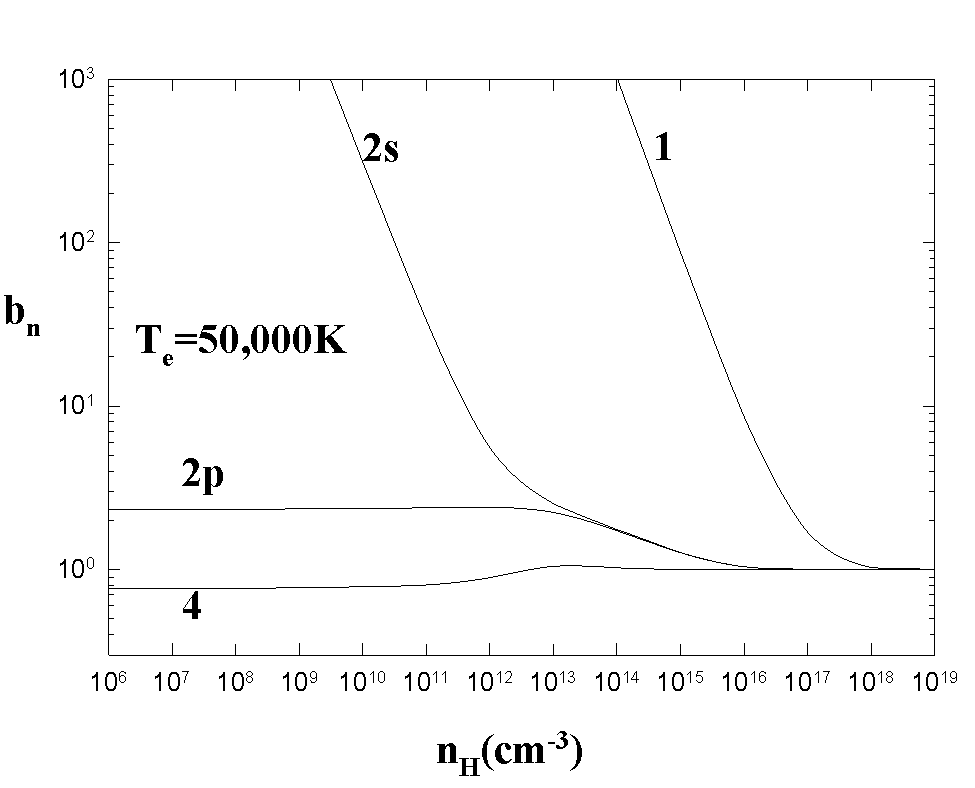
\includegraphics[scale=0.8]{Hmi_vs_density}
\caption[\hminus\ departure coefficients vs density]{Departure coefficients for \hminus\ are shown. The radiation density
was low and the total hydrogen density varied.  Three gas temperatures are
shown.  Collisions bring \hminus\ to LTE at high densities.}
\label{fig:Hmi_vs_density}
\end{figure}

For the majority of the calculations hydrogen is largely neutral, and
for the smaller temperatures a significant fraction of the hydrogen was
in the molecular form (H$_2$ and H$_2^+$).  The calculation confirms that the
departure coefficients are within 2\% of unity at the highest densities
computed.

\section{The HeH$^+$ molecular ion }

Rates for radiative association of He and H$^+$ to form HeH$^+$ are taken from \citet{Zygelman1990}.

\section{Linearization of the balance equations}

In the case of a molecular balance equation it is common to have a single
reaction that is the product of two unknowns.  The code works by complete
linearization, and uses the following scheme to produce a linear chemical
network.

Suppose we have two molecules with abundance $a$ and $b$, and with previous
abundances $a_o$ and $b_o$.  Then $\delta a = a - {a_o};\;\delta b = b -
{b_o}$ and the cross terms, $ab$, can be written as
\begin{equation}
\begin{array}{ccc}
 ab& =& \left( {{a_o} + \delta a} \right)\left( {{b_o} + \delta b} \right) \\
&\approx& {a_o}\delta b + {b_o}\delta a + {a_o}{b_o} \\
&\approx& {a_o}\left( {b - {b_o}} \right) + {b_o}\left( {a - {a_o}} \right)
+ {a_o}{b_o} \\
& =& {a_o}b + a{b_o} - {a_o}{b_o} \\
 \end{array}
\end{equation}

\section{The H$_2$ molecule}

The treatment of the hydrogen is described in \citet{Shaw2005}.  Other
details are in \citet{Ferland1989},
\citet{Ferland1994}, \citet{FerlandFabian2002}, and \citet{Abel2005}, while \citet{Roellig2007} compare
predictions of various codes.

\subsection{Stoichiometry}

The time dependent form of a reaction can be written as
\begin{equation}
\frac{{\partial {n_i}}}{{\partial t}} = {n_j}{R_f} - {n_i}{R_d}
\end{equation}
where $R_f$ is the rate that species with density $n_i$ is created from a species
with density $n_j$, and $R_d$ is the rate that $n_i$ is destroyed.  In the case of
hydrogen in the interstellar medium, the dominant formation process is
catalysis on grain surfaces, and the dominant destruction process is
photodissociation by the Solomon process.  This reaction corresponds to
the process $2n\left( {{{\mathrm{H}}^0}} \right) \to n\left( {{{\mathrm{H}}_2}}
\right)$
 and H$^0$ is removed from the gas at twice the rate that H$_2$ is formed.  The
balance equation is
\begin{equation}
\label{eqn:H2FormationBlance}
\frac{{\partial {n_i}}}{{\partial t}} = \frac{1}{2}n\left( {{{\mathrm{H}}^0}}
\right)n\left( {{{\mathrm{H}}^0}} \right){R_f} - n\left( {{{\mathrm{H}}_2}}
\right){R_d}.
\end{equation}

The convention in physical chemistry is to include only microphysical
processes in a reaction rate coefficient $R$, and to explicitly write the
stoichiometric factors in the equation, as done in equation \ref{eqn:H2FormationBlance}.

Tragically, the convention is astrophysics is to write the balance
equation as $n\left( {{{\mathrm{H}}^0}} \right)n\left( {{{\mathrm{H}}^0}}
\right){R_f} = n\left( {{{\mathrm{H}}_2}} \right){R_d}$
and absorb the stoichiometric factor of $\frac{1}{2}$ into the rate
coefficient.  So, the standard or \citet{Jura1974}, \citet{Jura1975} rate of H$_2$ formation
of grain surfaces, $3\times 10^{-17}$~cm$^3$~s$^{-1}$ at 100 K, includes a stoichiometric factor
of $\frac{1}{2}$.

\subsection{Associative detachment of \hminus}

The process
\begin{equation}
{{\mathrm{H}}^ - } + {\mathrm{H}} \Rightarrow {{\mathrm{H}}_2} + e
\end{equation}
is the main H$_2$ formation mechanism in low-density grain-free regions, and
is treated as described above.
At temperatures of interest here $(\sim 10^3 \K$)
the rate for H$_2$ formation by this process is set by the rate for radiative
association to form \hminus, and is of order 10$^{-15}$ cm$^3$ s$^{-1}$ (see above).

\subsection{Catalysis on grain surfaces}

The process
\begin{equation}
2{\mathrm{H}} + {\mathrm{grain}} \Rightarrow {{\mathrm{H}}_2} + {\mathrm{grain}}
\end{equation}
is a competitive H$_2$ formation process when grains are present.  The rate
coefficient is taken from \citet{Hollenbach1979} and \citet{Cazaux2002}.  Defining the fraction of atoms which form molecules as
\begin{equation}
{f_a} = {\left( {1 + {{10}^4}\exp \left( { - 600/{T_{gr}}} \right)}
\right)^{ - 1}}
\end{equation}
then the rate coefficient is given by
\begin{equation}
{\alpha _{gr}}\left( {{{\mathrm{H}}_2}} \right) = 3 \times {10^{ -
18}}\frac{{\sqrt T {A_{gr}}\,{f_a}}}{{1 + 0.04\sqrt {{T_{gr}} + T}  + 0.002T
+ 8 \times {{10}^{ - 6}}T_{}^2}}\quad
[\mathrm{cm}^3 \mathrm{s}^{-1}]
\end{equation}
where $A_{gr}$ is the grain abundance relative to the ISM value, and $T$
and $T_{gr}$
are the electron and grain temperatures respectively.  The grain temperature
is determined self-consistently, including radiative and collisional heating
and cooling, as described in the section \cdSectionTitle{Grain Physics}.

At $T=10^3 \K$ and $T_{gr}=100 \K$ (representative values of the gas and grain
temperature in regions near a H$^0 - \mathrm{H}_2$ interface) the rate coefficient for
grain catalysis is $\sim 4\times 10^{-18}$~cm$^{-3}$~s$^{-1}$.  For most conditions where
carbon is at least once ionized radiative association through \hminus\ is at least
a competitive H$^2$ formation mechanism.  The ratio of the two processes
(referred to as the \hminus\ and grain H$_2$ formation routes) is then
\begin{equation}
\frac{{r\left( {{{\mathrm{H}}^ - }} \right)}}{{r\left( {{\mathrm{grain}}} \right)}}
= \frac{{{n_e}\alpha \left( {{{\mathrm{H}}^ - }} \right)}}{{{n_H}\alpha \left(
{{\mathrm{grain}}} \right)}} \approx \frac{{{n_e}}}{{{n_H}}}250
\end{equation}
i.e., the \hminus\ route is faster for conditions of moderate ionization
($n_e/n_{\mathrm{H}}>4\times 10^{-3}$) even when grains are present.  When grains are absent (or
deficient) the \hminus\ route dominates.

\subsection{Excited atom radiative association}

Rates for the process
\begin{equation}
{\mathrm{H}}\left( {n = 2} \right) + {\mathrm{H}}\left( {n = 1} \right) \Rightarrow
{{\mathrm{H}}_2} + h\nu
\end{equation}
are taken from \citet{Latter1991}.

\subsection{Excited molecular dissociation}

Rates for the process
\begin{equation}
{{\mathrm{H}}_2}\left( {v \ge 4} \right) + {e^ - } \Rightarrow {\left(
{{\mathrm{H}}_2^ - } \right)^*} \Rightarrow {\mathrm{H}} + {{\mathrm{H}}^ - }
\end{equation}
are given in \citet{Janev1987} (their process 2.2.17), and these have been
adopted by \citet{Lenzuni1991} and \citet{Crosas1993} in their
work on high density gas.  Tests show that this process, if taken at face
value, is by far the fastest destruction mechanism for molecular hydrogen
under ISM conditions.

The process outlined by \citet{Janev1987} involves an electron capture
by H$_2$ into vibrationally excited levels ($4 \le v \le 9$).   The process is fast
at low temperatures because the energy barrier is small, and the excited
levels have large populations at laboratory densities.  The process proceeds
much more slowly at ISM densities, however, because excited levels have
populations below their LTE value.  This situation is thus similar to that
described by \citet{Dalgarno1979}.  We have modified the \citet{Janev1987} rates using the physics outlined by \citet{Dalgarno1979}.

\subsection{Collisional dissociation by H$^0$, He$^0$, and e$^-$}

The rate coefficient for the forward process, collisional dissociation
by the species S (one of H$^0$, He$^0$, or e$^-$),
\begin{equation}
{{\mathrm{H}}_2} + S \Rightarrow 2{\mathrm{H}} + S
\end{equation}
is taken from \citet{Dove1986} (dissociation by H$^0$),
\citet{Dove1987} (dissociation by He$^o$) and \citet{Janev1987} (dissociation by electrons).
These can be important destruction mechanisms only for warm regions of the
ISM because of the large binding energy of H$_2$ ($\sim$50,000~K).

The reverse reactions are included via detailed balance. Three-body
formation of H$_2$ is important only for very high densities [$n\cong
10^{10}$~cm$^{-3}$].

\section{Heavy element molecules}

\subsection{Cooling}

Cooling due to collisional excitation of vibration-rotation levels of
CH, OH, and H$_2$O is treated using the scheme outlined by HM79.

Of these CO is the most important. $^{12}$CO and $^{13}$CO are treated as
multi-level rigid rotors, with the full spectrum of the ground vibration
state predicted.


